\documentclass[border=10pt]{standalone}

\usepackage{tikz}
\usepackage{tikzsymbols}
\usetikzlibrary{calc,patterns,shapes.geometric}

\def\centerarc[#1](#2)(#3:#4:#5){\draw[#1] ($(#2)+({#5*cos(#3)},{#5*sin(#3)})$) arc (#3:#4:#5);}

\begin{document}
	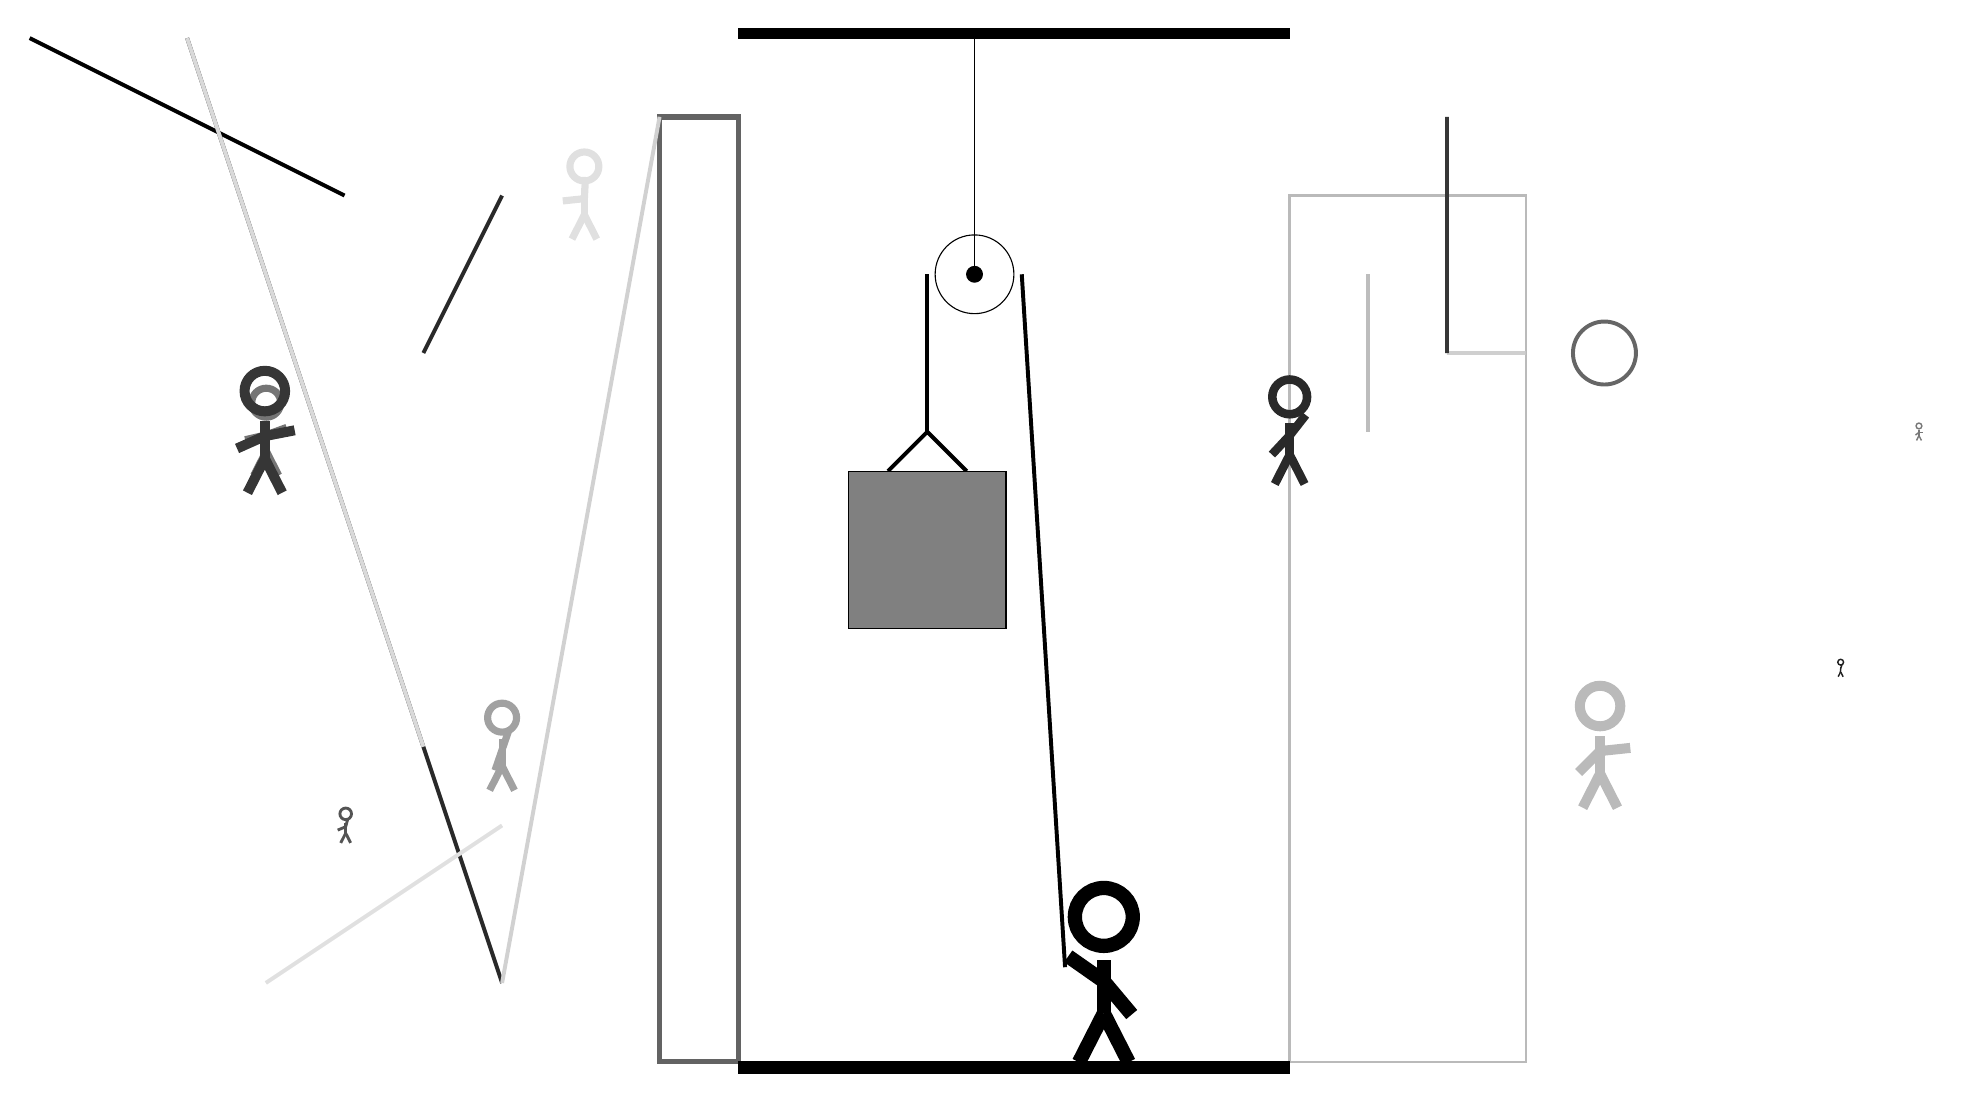
\begin{tikzpicture}
		%%%%% START %%%%%
		
		\draw[fill=black] (-2, 10) rectangle (5, 10.125);
		
		\draw [line width=0.5mm, color=black!60](9, 6) circle (0.4);
		
		\node[line width=0.4mm, color=black!27] at (9, 1) {\Strichmaxerl[7][45][6]};
		\node[line width=0.6mm, color=black!54] at (-8, 5) {\Strichmaxerl[5][13][20]};
		\node[line width=0.2mm, color=black!53] at (13, 5) {\Strichmaxerl[1][37][0]};
		\node[line width=0.4mm, color=black!37] at (-5, 1) {\Strichmaxerl[5][71][71]};
		\draw[line width=0.3mm, color=black!27] (5, 8) rectangle (8, -3);
		
		\node[line width=0.2mm, color=black!12] at (-4, 8) {\Strichmaxerl[5][6][87]};
		\draw[line width=0.5mm, color=black!84](-5, -2) -- (-9, 10);
		\draw[line width=0.7mm, color=black!61] (-2, -3) rectangle (-3, 9);
		\draw[line width=0.5mm, color=black!84](-6, 6) -- (-5, 8);
		\draw[line width=0.5mm, color=black!26](6, 7) -- (6, 5);
		\draw[line width=0.5mm, color=black!12](-5, 0) -- (-8, -2);
		\draw[line width=0.4mm, color=black!19] (7, 6) rectangle (8, 6);
		
		\draw[line width=0.5mm, color=black!100](-7, 8) -- (-11, 10);
		\node[line width=0.3mm, color=black!84] at (5, 5) {\Strichmaxerl[6][47][52]};
		\draw[line width=0.5mm, color=black!18](-3, 9) -- (-5, -2);
		
		\draw[line width=0.5mm, color=black!15](-6, 1) -- (-9, 10);
		\draw[line width=0.6mm, color=black!79] (7, 6) rectangle (7, 9);
		\node[line width=0.4mm, color=black!67] at (-7, 0) {\Strichmaxerl[2][23][75]};
		
		\node[line width=0.5mm, color=black!79] at (-8, 5) {\Strichmaxerl[7][24][11]};
		\node[line width=0.3mm, color=black!88] at (12, 2) {\Strichmaxerl[1][86][71]};
		
		
		\draw (1, 7) circle (0.5);
		\draw[fill=black] (1, 7) circle (0.1);
		\draw (1, 10) -- (1, 7);
		
		\draw[line width=0.5mm] (-0.1, 4.5) -- (0.4, 5.0) -- (0.9, 4.5);
		\draw[fill=black!50] (-0.6, 4.5) rectangle (1.4, 2.5);
		
		\draw[line width=0.5mm] (0.4, 7) -- (0.4, 5.0);
		\centerarc[line width=0.5mm](1, 7)(0:180:0.6);
		\draw[line width=0.5mm](1.6, 7) -- (2.15, -1.8);
		
		\node at (2.6, -1.9) {\Strichmaxerl[10][-35][-50]};
		
		\draw[fill=black] (-2, -3) rectangle (5, -3.15);
		
		%%%%% END %%%%%
	\end{tikzpicture}
\end{document}